\documentclass[11pt]{article}
\usepackage[utf8]{inputenc}
\usepackage[brazilian]{babel}

\usepackage{subfigure}
\usepackage{indentfirst}
\usepackage{graphicx}
\usepackage{xcolor}
\usepackage[cm]{fullpage}
\usepackage{hyperref}
\usepackage{listings}
\lstset{
  basicstyle=\footnotesize\ttfamily,
}

\newcommand*{\alert}[1]{\vspace{0.4cm}\colorbox{gray!60!white}{\parbox{0.92\linewidth}{{\centering \textbf{IMPORTANTE!}\\}#1}}\vspace{0.4cm}}

\title{Guia Básico do Nanvix: Instação, Compilação, Execução e Depuração}

\author{Pedro H. Penna, Fernando Jorge Mota e Márcio Castro\\[0.3em]
\small Universidade Federal de Santa Catarina}
\date{}

\hyphenation{tool-chain}

\usepackage{url}

\begin{document}

\maketitle

\section{Introdução}

Antes de começar a \textit{hackear} o Nanvix, é fundamental que você se familiarize com o modo como os arquivos do projeto estão organizados, com quais ferramentas de desenvolvimento você vai lidar e com o processo de compilação. Nesse primeiro projeto, você vai trabalhar em todas essas tarefas e, ao final, estará pronto para começar o trabalho duro.

É importante notar os scripts fornecidos para instalação e execução do Nanvix foram testados em distribuições Ubuntu e Lubuntu. Portanto, recomendamos fortemente que você utilize uma dessas duas distribuições. Certamente o Nanvix poderá ser compilado e executado em outras distribuições. Porém, será preciso em alguns casos realizar modificações nos scripts de instalação. 

Inicialmente mostraremos como baixar o código fonte do Nanvix e discutiremos sua estrutura de diretórios (Seção~\ref{sec:codigo}). Em seguida, mostraremos como instalar as ferramentas de desenvolvimento que permitirão a sua compilação (Seção~\ref{sec:ferramentas}). Posteriormente, mostraremos como compilar e executar o Nanvix (Seção~\ref{sec:compilacao}). Então, apresentaremos uma maneira interessante de depurar o Nanvix com uso do GDB (Seção~\ref{sec:debug}). Por fim, mostraremos duas alternativas de utilização do Nanvix através do uso de Máquinas Virtuais (VMs): em uma máquina local (Seção~\ref{sec:vm}) e na nuvem (Seção~\ref{sec:vm-ufsc}).

\section{Código Fonte e Estrutura do Projeto}
\label{sec:codigo}
O primeiro passo para utilizar o Nanvix é baixar o seu código fonte. Para isso, basta clonar o seu repositório de desenvolvimento da seguinte forma\footnote{Caso você não tenha o \texttt{git} instalado, você poderá instalá-lo da seguinte forma: \texttt{sudo apt-get install git}}:\\

\begin{lstlisting}[language=bash,numbers=none,frame=single]
git clone https://github.com/nanvix/nanvix
\end{lstlisting}

\vspace{0.3cm}
Dentro do diretório do Nanvix você encontrará uma série de arquivos e diretórios. Por tratar-se de um projeto ligeiramente grande e complexo, o Nanvix é organizado em uma hierarquia de diretórios, que é detalhada a seguir:

\begin{itemize}
    \item \texttt{bin} conterá o binário do \textit{kernel} e utilitários, depois de terem sido compilados.
    \item \texttt{doc} contém toda a documentação do Nanvix, que inclui manuais do sistema, de bibliotecas e utilitários; orientações gerais para desenvolvimento; e documentação de APIs.
    \item \texttt{doxygen} contém arquivos de configuração da ferramenta Doxygen, que gera documentação das APIs do Nanvix diretamente do código fonte.
    \item \texttt{include} contém os arquivos-cabeçalhos de escopo global, tanto de sistema quanto de biblioteca.
    \item \texttt{lib} conterá todas as bibliotecas estáticas e dinâmicas, depois de terem sido compiladas.
    \item \texttt{src} contém o código fonte do Nanvix.
    \item \texttt{tools} contém todas as ferramentas e \textit{scripts} necessários para compilar o Nanvix.
\end{itemize}

\section{Instalação das Ferramentas e Ambiente de Desenvolvimento}
\label{sec:ferramentas}

As ferramentas utilizadas no desenvolvimento do Nanvix, como no desenvolvimento de qualquer outro sistema operacional, se diferem das utilizadas no desenvolvimento da maioria dos outros tipos de software. Em primeiro lugar, as ferramentas de compilação devem ser compatíveis com a plataforma alvo. Por exemplo, o Nanvix foi projetado para a plataforma x86, portanto as ferramentas utilizadas para compilar o sistema devem ser capazes de gerar código de máquina para essa plataforma. Em segundo lugar, quando trabalha-se em nível de \textit{kernel}, o ambiente de desenvolvimento não provê quaisquer tipo de bibliotecas padrões. Em terceiro lugar, para testar o sistema deve-se utilizar uma máquina dedicada, seja ela real ou virtual. Finalmente, em quarto lugar, as ferramentas de \textit{debugging} disponíveis são restritas.

Para o desenvolvimento do Nanvix, você utilizará duas ferramentas: a \textit{toolchain} GCC-x86, uma coletânea de utilitários que inclui compilador, \textit{assembler} e \textit{linker}; e o \textit{Bochs}, um emulador para plataforma x86. Para instalar as ferramentas de forma automática execute os seguintes comandos \textbf{a partir do diretório raiz do projeto}: \\

\begin{lstlisting}[language=bash,numbers=none,frame=single]
sudo apt-get install make
sudo bash tools/dev/setup-toolchain.sh
sudo bash tools/dev/setup-bochs.sh
sudo reboot now
\end{lstlisting}

\vspace{0.3cm}
É esperado que o processo de instalação das ferramentas demore um certo tempo (vários minutos).

\section{Compilação e Execução}
\label{sec:compilacao}

Uma vez que as ferramentas de desenvolvimento necessárias para compilar o Nanvix foram devidamente instaladas, compilar o sistema torna-se uma tarefa simples. Do diretório raiz do projeto, invoque os seguintes comandos \textbf{a partir do diretório raiz do projeto}:\\

\begin{lstlisting}[language=bash,numbers=none,frame=single]
make nanvix
make image
\end{lstlisting}

\vspace{0.3cm}
O primeiro comando realiza a compilação do Nanvix. Terminado esse processo, todos os binários devem ter sido criados com sucesso. O segundo comando gera uma imagem\footnote{Se você usa a distribuição \textit{Arch Linux} talvez seja necessário instalar o pacote \texttt{cdrtools} para criar a imagem. Para isso, execute o seguinte comando: \texttt{pacman -S cdrtools}} do sistema, criando-se assim o arquivo \texttt{nanvix.img} no diretório raiz. Esse arquivo é a imagem do sistema e será usado no processo de \textit{boot}, a seguir.

Finalmente, inicie o Nanvix no \textit{Bochs}, dando \textit{boot} pela imagem de sistema gerada. Para fazer isso de forma automática, execute o seguinte comando \textbf{a partir do diretório raiz do projeto}:\\

\begin{lstlisting}[language=bash,numbers=none,frame=single]
bash tools/run/run.sh
\end{lstlisting}

\vspace{0.3cm}
Pronto! Em caso de sucesso, você verá o Nanvix sendo inicializado. Após a inicialização, a tela principal do terminal do Nanvix está pronta para utilização, conforme mostra a Figura~\ref{fig:terminal-nanvix}.

\begin{figure}[t]
	\centering
	\subfigure[Nanvix após inicialização.]{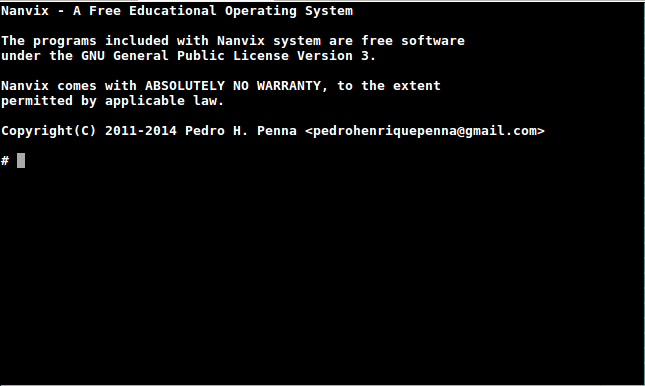
\includegraphics[scale=0.38]{img/terminal-nanvix.png}\label{fig:terminal-nanvix}}
	\subfigure[GDB após um \textit{breakpoint} na função \texttt{yield()} do \textit{kernel}.]{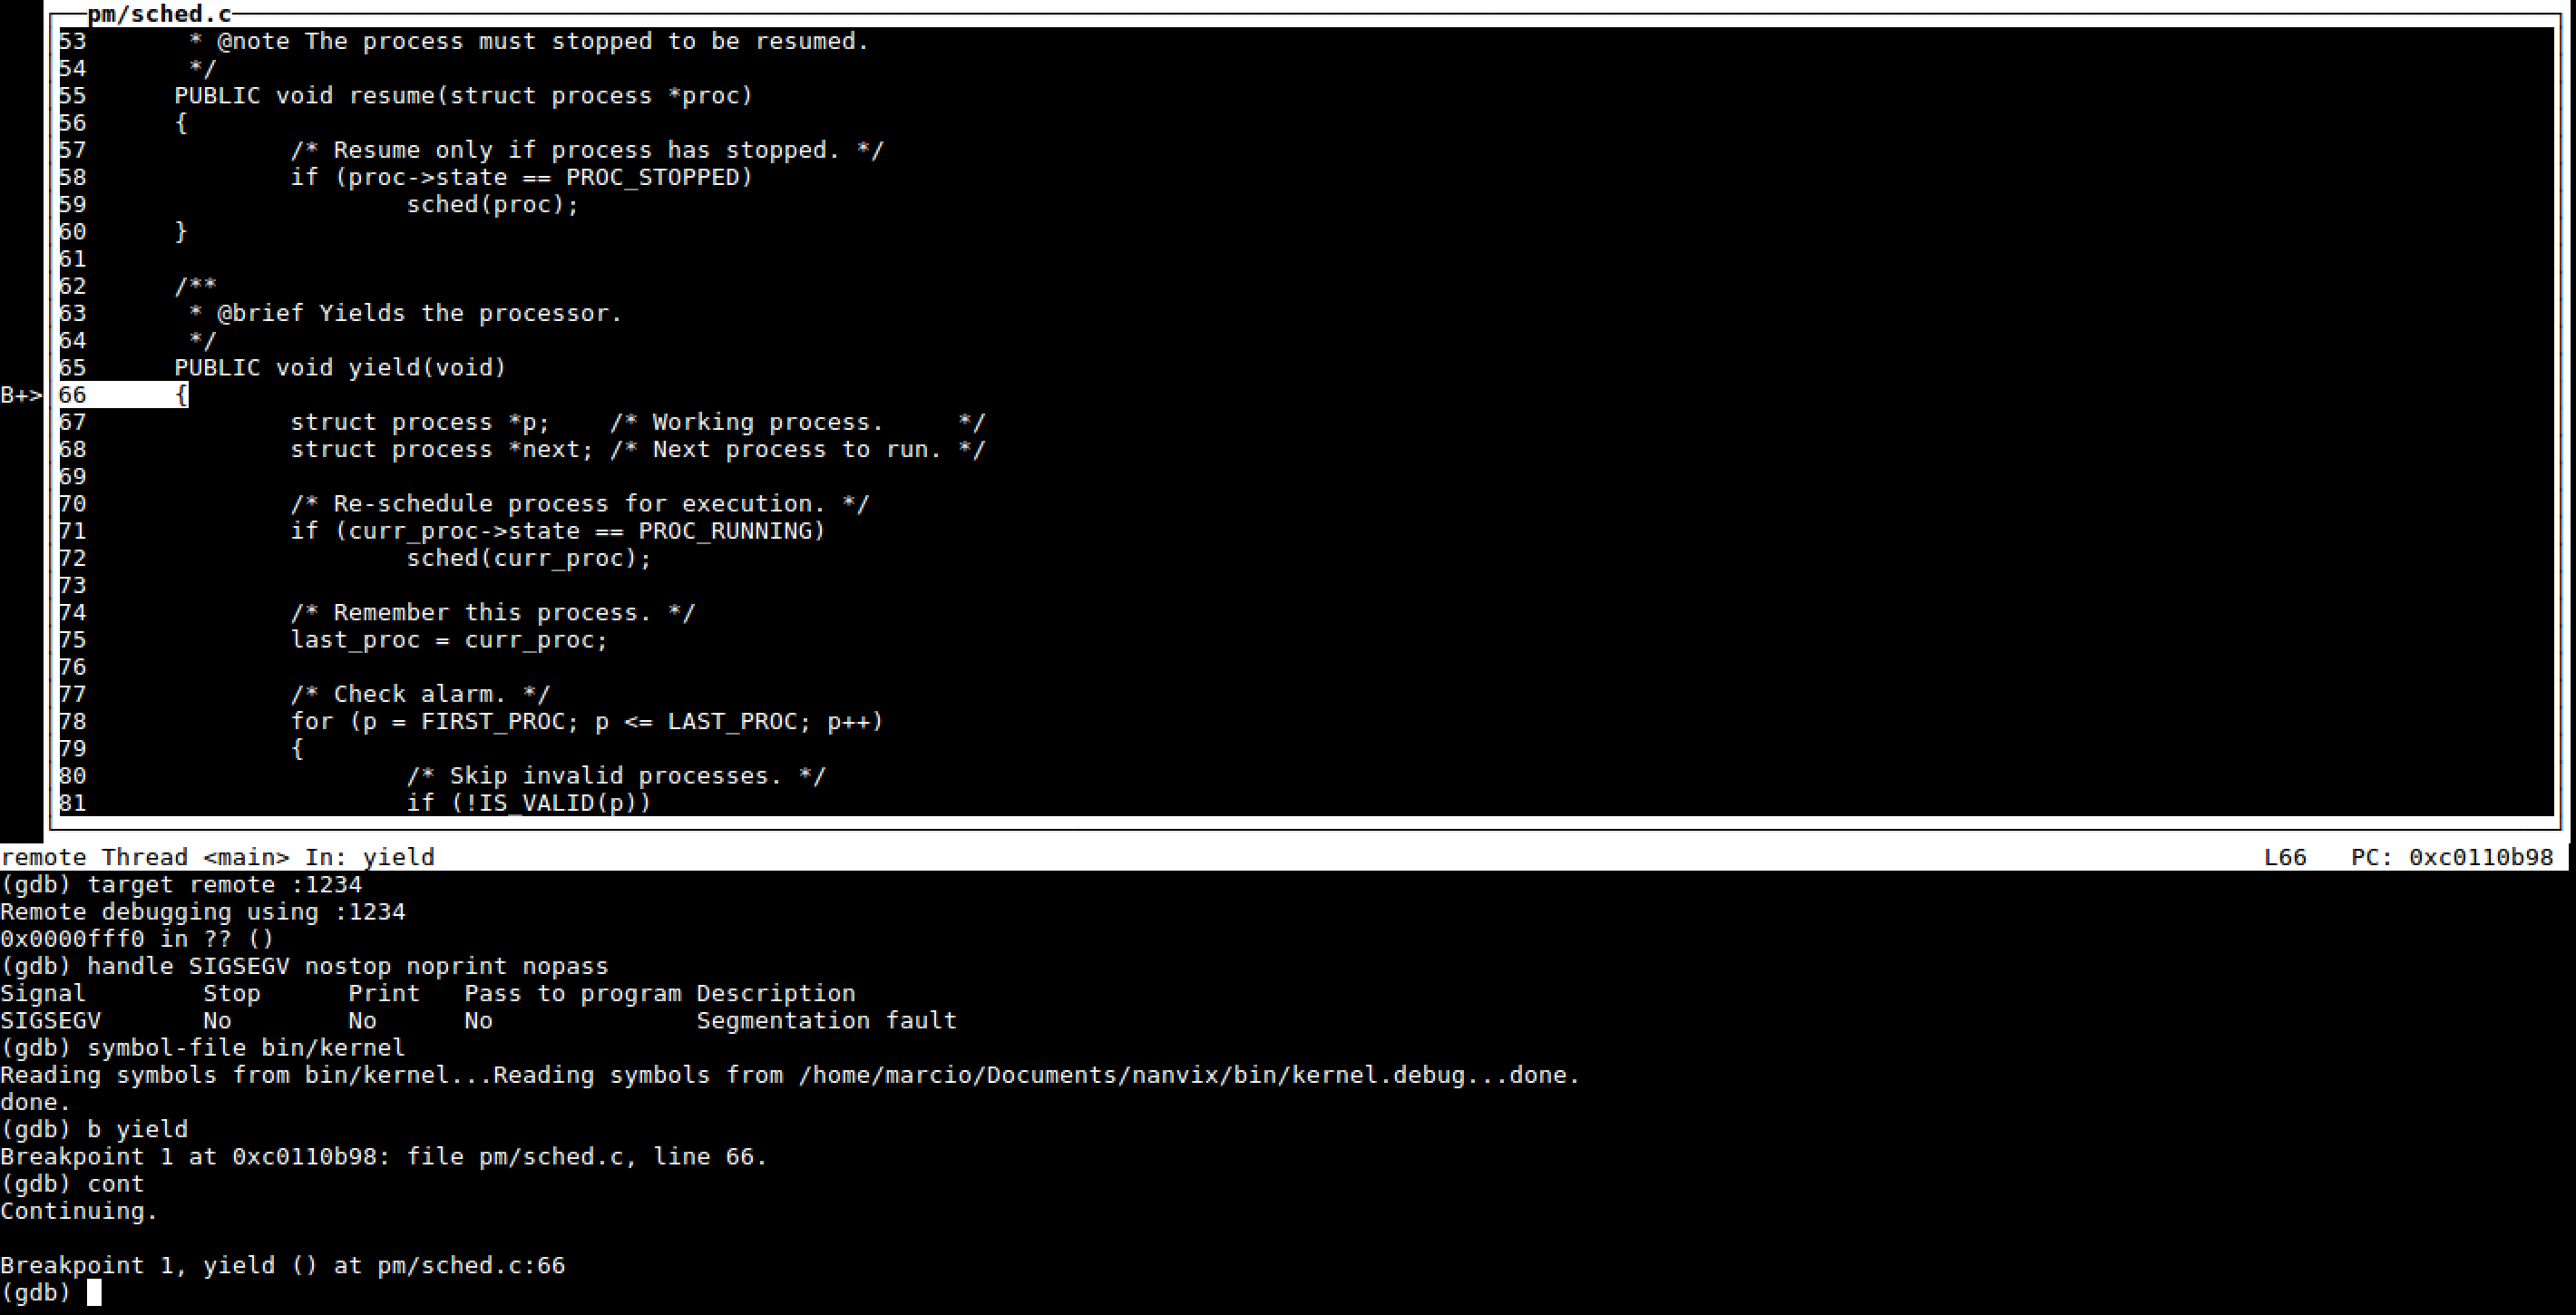
\includegraphics[scale=0.22]{img/terminal-GDB.png}\label{fig:terminal-gdb}}
\caption{Terminais do Nanvix e do GDB.}
\end{figure}

\alert{O \textit{Bochs} será executado diretamente na tela do terminal. Para finalizar a execução do emulador \textit{Bochs} corretamente, pressione primeiramente CTRL+Z para pausar a execução do processo \textit{Bochs}. Então, digite o seguinte comando no terminal para finalizar a execução do \textit{Bochs}: \texttt{kill -HUP \%1}.}

\section{Depurando o Nanvix}
\label{sec:debug}

Para depurar Nanvix, o que pode ser muito útil na resolução de \textit{bugs} e outros problemas que surgirão durante o desenvolvimento de código no \textit{kernel}, será necessário o uso do GDB, cujo uso e integração serão definidos nessa seção. Caso você esteja numa conexão remota (e.g., usando \texttt{ssh}), é extremamente sugerido o uso do \texttt{tmux} para evitar a necessidade de criar mais de uma conexão \texttt{ssh}, visto que quando o \textit{Bochs} está rodando ele assume o comando do terminal inteiro. Nesse caso, instale o \texttt{tmux} usando o comando \texttt{sudo apt-get install tmux}. Após a instalação, execute o comando \texttt{tmux} e pressione CTRL+B+\% para abrir dois \textit{panes}. Em seguida, use CTRL+B+(seta para direita ou seta para a esquerda) para alterar livremente entre os terminais. Mais informações podem ser vistas diretamente no manual do \texttt{tmux} disponível em: \url{https://leanpub.com/the-tao-of-tmux/read}.

Para rodar o Nanvix em modo depuração (\textit{debug}) e ativar o suporte ao GDB utilize o seguinte comando em um terminal: \\

\begin{lstlisting}[language=bash,numbers=none,frame=single]
bash tools/run/run.sh --debug
\end{lstlisting}

\vspace{0.3cm}
Depois, inicialize o GDB \textbf{em um outro terminal} a partir do diretório raiz do projeto, usando o seguinte comando: \\

\begin{lstlisting}[language=bash,numbers=none,frame=single]
gdb --tui
\end{lstlisting}

O argumento \texttt{--tui} é opcional mas muito interessante. Com ele você habilitará o suporte a uma interface de usuário de modo texto para visualizar o código fonte durante a depuração, como mostrado na Figura~\ref{fig:terminal-gdb}.
\newpage
Para começar a depurar, execute os seguintes comandos no terminal do GDB:\\

\begin{lstlisting}[language=sh,numbers=none,frame=single]
target remote :1234
handle SIGSEGV nostop noprint nopass
cont
\end{lstlisting}

\vspace{0.3cm}
Segue uma explicação breve aos comandos informados acima:

\begin{enumerate}
	\item Conecta-se ao \textit{Bochs}, que agora mostrará que há um cliente conectado;
	\item Define que \textit{page faults} e outras interrupções frequentes devem ser ignoradas completamente pelo GDB. O \texttt{SIGSEGV} aqui é apenas um \textit{alias} para representar essas outras interrupções que são normais durante a execução da máquina;
	\item Define que a máquina deve continuar sua execução.
\end{enumerate}

Pronto! Em caso de sucesso você verá o GDB conectado ao \textit{Bochs}, como mostra a Figura~\ref{fig:terminal-gdb}. Após a execução do comando \texttt{cont}, o terminal do Nanvix ficará disponível na tela do \textit{Bochs} e o \textbf{GDB ficará bloqueado}. Para liberar o terminal do GDB novamente, aperte \textbf{CTRL+C} no terminal do GDB. Dessa forma, o GDB pausará a execução do Nanvix novamente e permitirá o controle da execução em modo \textit{debug} através do GDB.

Durante a compilação do Nanvix, diversos arquivos contendo as tabelas de símbolos de funções do \textit{kernel} e de programas de sistema e de usuário são criados. Porém, essas tabelas de símbolos não são carregadas automaticamente. Para carregar a tabela de símbolos contendo informações sobre todas as funções do \textit{kernel}, você pode usar o comando:\\

\begin{lstlisting}[language=sh,numbers=none,frame=single]
symbol-file bin/kernel
\end{lstlisting}

\vspace{0.3cm}
Alternativamente, se o seu objetivo for depurar algum programa específico dentro do Nanvix será necessário carregar a tabela de símbolos do programa desejado. Por exemplo, para carregar a tabela de símbolos do programa \texttt{ls}, informe o caminho para o executável dentro da pasta \texttt{bin}:\\

\begin{lstlisting}[language=sh,numbers=none,frame=single]
symbol-file bin/ubin/ls
\end{lstlisting}

\alert{Não é recomendável usar mais de uma tabela de símbolos ao mesmo tempo, pois nesse caso o GDB não será capaz de diferenciar corretamente os símbolos. Logo, ao realizar esse comando em um terminal onde a tabela de símbolos do \textit{kernel} já foi carregada o GDB perguntará se a tabela de símbolos deve ser substituída, o que é necessário para depurar um programa do Nanvix.}

Para definir \textit{breakpoints}, você pode usar o comando \texttt{b} \textbf{depois da tabela de símbolos ser carregada}. Para depurar a função \texttt{yield}, por exemplo, é possível simplesmente fazer:\\

\begin{lstlisting}[language=sh,numbers=none,frame=single]
b yield
\end{lstlisting}

\vspace{0.3cm}
No lugar do nome da função, você pode também definir uma linha onde o GDB deve definir o \textit{breakpoint}. Dessa forma, você pode usar o seguinte comando para definir um \textit{breakpoint} na linha 143 do arquivo \textbf{main.c}, por exemplo:\\

\begin{lstlisting}[language=sh,numbers=none,frame=single]
b main.c:143
\end{lstlisting}

\vspace{0.3cm}
Observe que a função de \textit{breakpoint} só funciona bem se você carregar a tabela de símbolos usando o comando \texttt{symbol-file}, anteriormente especificado, pois é a partir da tabela de símbolos que o GDB consegue identificar os arquivos e funções envolvidos.

Após especificar um \textit{breakpoint}, você poderá utilizar o comando \texttt{cont} para informar o GDB que o mesmo deve parar ao acontecer a próxima ocorrência de qualquer \textit{breakpoint} anteriormente definido. Então, a partir de um determinado \textit{breakpoint}, é possível usar o comando  \texttt{step} para saltar para a próxima instrução:\\

\begin{lstlisting}[language=sh,numbers=none,frame=single]
step
\end{lstlisting}

\vspace{0.3cm}
Você também pode saltar um número definido de instruções com uso de um parâmetro opcional do \texttt{step}. Por exemplo, utilize o seguinte comando para saltar 10 instruções de uma única vez:\\

\begin{lstlisting}[language=sh,numbers=none,frame=single]
step 10
\end{lstlisting}

\vspace{0.3cm}
O comando \texttt{step} permite realizar uma depuração do tipo \textit{step-by-step}. Isso significa que quando uma função é invocada durante a depuração, o GDB fará o desvio para a primeira instrução dentro da função. Caso você queira saltar diretamente para o retorno da função antes de invocá-la, você poderá utilizar o comando \texttt{next}:\\

\begin{lstlisting}[language=sh,numbers=none,frame=single]
next
\end{lstlisting}

\vspace{0.3cm}
Além disso, durante a depuração, é interessante usar o comando \texttt{print} para imprimir variáveis que possam ser úteis para entender a execução do código. Dessa forma, para imprimir a variável global \texttt{curr\_proc}, que está presente no \textit{kernel} do Nanvix, é possível usar:\\

\begin{lstlisting}[language=sh,numbers=none,frame=single]
print curr_proc
\end{lstlisting}

Da mesma forma, é possível usar parte da sintaxe do C para explorar os diferentes atributos que a variável possa ter. Por exemplo, para imprimir o atributo \texttt{pid} de \texttt{curr\_proc}, faça:\\

\begin{lstlisting}[language=sh,numbers=none,frame=single]
print curr_proc->pid
\end{lstlisting}

\vspace{0.3cm}
O comando acima imprime o PID do processo atual em execução (no caso do Nanvix, o PID é um atributo de \texttt{curr\_proc}). Observe que o \texttt{print} também funciona em \textit{breakpoints}, com variáveis locais, sendo portanto bastante útil para entender o que está acontecendo no código.

Por fim, para saber a sequência de chamadas atual, você pode usar o comando \texttt{bt}, que imprime o \textit{back-trace} atual do código:\\

\begin{lstlisting}[language=sh,numbers=none,frame=single]
bt
\end{lstlisting}

\vspace{0.3cm}
Para mais informações a respeito do GDB, consulte o manual em: \url{https://sourceware.org/gdb/current/onlinedocs/gdb/}

\alert{O \textit{Bochs} não suporta determinadas operações que o GDB suporta, como \texttt{watch} (para acompanhar o valor de uma variável ao longo do tempo), ou chamadas de função no \texttt{print}. Fazer isso resulta em erro, em uma instabilidade do sistema ou ambos. Portanto, sua utilização não é recomendada.}

\section{Nanvix em uma Máquina Virtual (VM)}
\label{sec:vm}

Caso você não tenha uma máquina com Linux e não tenha interesse em instalá-lo diretamente na sua máquina, você poderá fazer uma instalação do Linux em uma Máquina Virtual (VM) rodando em um outro sistema operacional (e.g., Windows). Nesse caso, aconselhamos a utilização do \textit{Virtual Box}
(disponível em \url{www.virtualbox.org}). Após instalar o Virtual Box, aconselhamos a instalação do Lubuntu 16.04 (disponível em \url{http://lubuntu.net}) na VM, pois trata-se de uma distribuição relativamente leve e testada. Por fim, basta seguir os passos de instalação e compilação (Seções~\ref{sec:codigo} a~\ref{sec:compilacao}) do Nanvix no Lubuntu.

\section{Nanvix na Nuvem -- Servidor Virtual da UFSC}
\label{sec:vm-ufsc}

A SeTIC/UFSC disponibiliza um serviço \textbf{experimental} para as unidades acadêmicas e administrativas da UFSC como uma alternativa a hospedagem de um equipamento físico. A tecnologia de virtualização permite que múltiplas instâncias de servidores virtuais rodem de forma independente em um único servidor físico. Alunos matriculados na disciplina INE5412 tem direito a criar servidores virtuais nessa infraestrutura. Para criar um servidor virtual, siga os seguintes passos:

\begin{enumerate}
	\item Acesse o endereço \url{https://idufsc.ufsc.br/} e faça login com as suas credenciais da UFSC.
	\item No menu superior, clique em \textit{Nuvem}.
	\item Clique na aba \textit{Servidores Virtuais}.
	\item Clique no botão \textit{Criar servidor} para criar um servidor virtual. Dê um nome a ele e selecione a distribuição \textit{Ubuntu 14.04}.
	\item Após a criação do servidor, o sistema irá mostrar o seu \textit{username} e sua \textit{senha temporária}. Guarde estas informações, pois elas serão necessárias para acessar o servidor virtual.
	\item Clique no ícone \textit{play} para dar \textit{boot} no servidor virtual. O ícone \textit{play} ficará inativo quando o servidor virtual tiver sido iniciado.
\end{enumerate}

Pronto! O seu servidor virtual foi criado e iniciado. Agora, faça um acesso remoto ao seu servidor virtual utilizando \texttt{ssh} (substitua \texttt{<nome.servidor>} pelo nome do servidor virtual escolhido no passo 4 e \texttt{<seu.username>} pelo seu \textit{username} mostrado no passo 5). Quando a senha for requisitada, digite a senha temporária criada no passo 5:\\

\begin{lstlisting}[language=sh,numbers=none,frame=single]
ssh <seu.username>@<nome.servidor>.<seu.username>.vms.ufsc.br
\end{lstlisting}

\vspace{0.3cm}

Você está agora \textit{logado} remotamente em seu servidor virtual. A partir deste ponto, basta seguir os passos de instalação e compilação (Seções~\ref{sec:codigo} a~\ref{sec:compilacao}) do Nanvix. 

\alert{1 -- Por ser um serviço experimental, a SeTIC não se responsabiliza pela disponibilidade do serviço e pela segurança (\textit{backup}) dos seus dados.\\ \vspace{-0.2cm} \\ 2 -- Para acessar o seu servidor virtual fora da rede UFSC será necessário utilizar o serviço de VPN da UFSC. As instruções para a configuração da VPN UFSC estão disponíveis no seguinte endereço: \url{https://servicosti.sistemas.ufsc.br/publico/detalhes.xhtml?servico=112}.}

\end{document}
